\documentclass[../main.tex]{subfiles}
\makeatletter
\@ifundefined{fromRoot}{%
  \newcommand{\fromRoot}[1]{../#1}
  
  \usepackage{xr}
  \externaldocument{../main}
}{}

\def\input@path{{\subfix{../}}}
%or: \def\input@path{{/path/to/folder/}{/path/to/other/folder/}}
\makeatother

\graphicspath{{\subfix{../}}}

\hypersetup{
    pdfauthor   = {Mael Tourres},
    pdftitle    = {Th\`{e}se (Chapitre 2_2)},
    pdfsubject  = {Th\`{e}se (Chapitre 2_2)},
%    pdfkeywords = {mots-cl\'{e}s},
}

\begin{document}
\selectlanguage{french}
%
%
%
%
\chapter{Stratégies d'implantation des décodeurs de CCE} 
\label{chapter:2_2}
\chaptermark{Stratégies d'implantation des décodeurs de CCE}
%
%
%
%
%

Ce chapitre se focalise sur les architectures numériques et les systèmes utilisés pour intégrer ces différentes familles de CCE, sous contrainte temps réel dans des systèmes embarqués.
Les différentes stratégies d’implantation de ces CCE sont également présentées. Ces notions permettent de positionner ces travaux de thèse relativement à l'état de l'art et de préciser les motivations dans la dernière partie de ce chapitre.

%
%
%
%
%
%
%
\etocsetnexttocdepth{4}
\etocsettocstyle{
    { \large \hspace{-1.5 em} \textbf{} \hfill}
    \vspace{-2.5 em}\\\par\noindent\rule{\linewidth}{1 pt}\vspace{-.2 em}
    }
{\par\noindent\rule{\linewidth}{1 pt}\\}
\localtableofcontents

%
% 
% 
% 
% 
\section{Introduction}
% 
% 
% 
% 

Comme évoqué précédemment, les CCE sont présents dans la majorité des systèmes de communication et de stockage de l’information que nous utilisons. L'hétérogénéité des contextes applicatifs a abouti au développement et à la standardisation de nombreux codes différents.\\
L’implantation de décodeurs sous contrainte temps réel devient complexe pour les concepteurs, car différents paramètres sont à prendre en considération: complexité matérielle, débit, latence et/ou consommation énergétique. Afin d'adresser l’ensemble de ces besoins, différentes stratégies de parallélisation et d’implantation des décodeurs ont été imaginées et déployées sur différentes technologies matérielles \acrshort{asic}/\acrshort{fpga}. Par ailleurs, ces différentes stratégies ont été plus récemment investiguées sur des architectures programmables (CPU multicœurs et GPU). Lors de l’implantation d’un décodeur CCE, les diverses solutions proposées dans la littérature doivent être déclinées et optimisées afin de s’adapter aux paramètres algorithmiques du ou des codes sélectionnés et des contraintes applicatives aboutissant à un nombre important de solutions pour une seule famille de CCE. Deux types de paramètres contraignent fortement la conception des décodeurs :

    \textbf{Les paramètres algorithmiques} – ce sont les caractéristiques intrinsèques du code telles que la taille \textbf{N} des trames à décoder ainsi que le rendement \textbf{R} du code. D’autres caractéristiques propres à chaque famille affectent aussi la conception des décodeurs, comme la structure de la matrice de parité pour un code LDPC ou encore les positions des bits gelés pour un code polaire. Ces paramètres varient généralement d’un standard ou d’un cas d’usage à l’autre. 
    
    \textbf{Les paramètres architecturaux} – ce sont les caractéristiques d’implantation. Il peut s’agir du format de quantification des données internes au décodeur, du facteur de parallélisation des calculs, du nombre d’itérations de décodage pour un algorithme itératif, etc. Ces paramètres, dérivés des contraintes du système à concevoir, peuvent, pour certains, être issus de phases de raffinement et de simulation successives. Ils ont un impact direct sur l'architecture à concevoir et, par conséquent, sur la complexité matérielle et énergétique du décodeur.

La multiplicité des cadres applicatifs nécessite donc de disposer d’un large éventail d'implantations dans l’espace des solutions. Par exemple, dans le standard 3GPP 5G \cite{26}, le standard couvre des besoins allant de décodeurs soumis à de faibles débits pour des réseaux de capteurs \cite{27} à des décodeurs très hauts débits (quelques Gbit/s) pour des systèmes de vidéo transmission \cite{28}. En plus de ces cas extrêmes, d'autres contextes applicatifs, tels que celui des voitures autonomes \cite{29}, nécessitent des décodeurs à très faible latence. Cette hétérogénéité s’étend à d’autres paramètres liés à la nature des systèmes : les contraintes énergétiques ne sont pas homogènes entre des systèmes de type IoT \cite{30} et les infrastructures de type Cloud-RAN \cite{CLOUD:RAN1,CLOUD:RAN2,CLOUD:RAN3,INTEL:FLEXRAN} tout comme les besoins en termes de flexibilité et d’évolutivité des décodeurs intégrés dans ces systèmes.

En fonction de la nature des systèmes à concevoir, en plus des contraintes appliquées à ces derniers, différentes stratégies d’implantation sont actuellement mises en œuvre. Depuis quelques années, en parallèle de la conception d’architectures dédiées (ex. ASIC, FPGA), les implantations logicielles sur des cibles programmables (CPU multicœurs et GPU) sont devenues viables. Cela a été rendu possible grâce à l’évolution des architectures programmables qui offrent un niveau de flexibilité élevé au détriment des performances énergétiques. L’évolution des stratégies d’implantation des décodeurs CCE ainsi que des méthodologies de conception associées sont traitées dans les sections suivantes.
%
% 
% 
% 
% 
\section{Architectures dédiées}

Historiquement, l’implantation de chaînes de communications numériques, et donc de décodeurs de CCE, nécessitait la conception d’architectures numériques dédiées afin de respecter les contraintes applicatives, cela tant en termes de débits que de consommation énergétique. Ces architectures dédiées étaient décrites au niveau RTL \cite{17} dans des langages tels que le VHDL ou Verilog avant d’être synthétisées, placées et routées pour des technologies ASIC avant d'être produites en grande quantité dans des fonderies (figure \ref{methodo_archi_dediees}). En procédant ainsi, les concepteurs s’assuraient une maîtrise totale du système implanté, leur permettant, en fonction des besoins, soit de maximiser le débit, de minimiser la consommation énergétique ou bien de trouver des compromis entre ces paramètres. Ce contrôle total sur l’implantation permettait aussi l’usage de techniques d’optimisations fines en lien avec les capacités de la technologie ASIC ciblée. Ainsi, de nombreux décodeurs CCE, toutes familles de codes confondues, ont été réalisés \cite{AA1}. Malgré la complexité des méthodologies de conception et le temps nécessaire au développement et la production d’ASIC, cette approche est toujours plébiscitée pour les systèmes très contraints en termes de débits et/ou énergétiquement. Récemment, des décodeurs CCE qui atteignent des débits avoisinants 100 Gbps voire 1 Tbps ont notamment été décrits dans la littérature \cite{AA2, AA3, AA4}.

%%%%%%%%%%%%%%%%%%%%%%%%%%%%%%%%%%%%%%%
\begin{figure}
    \centering
    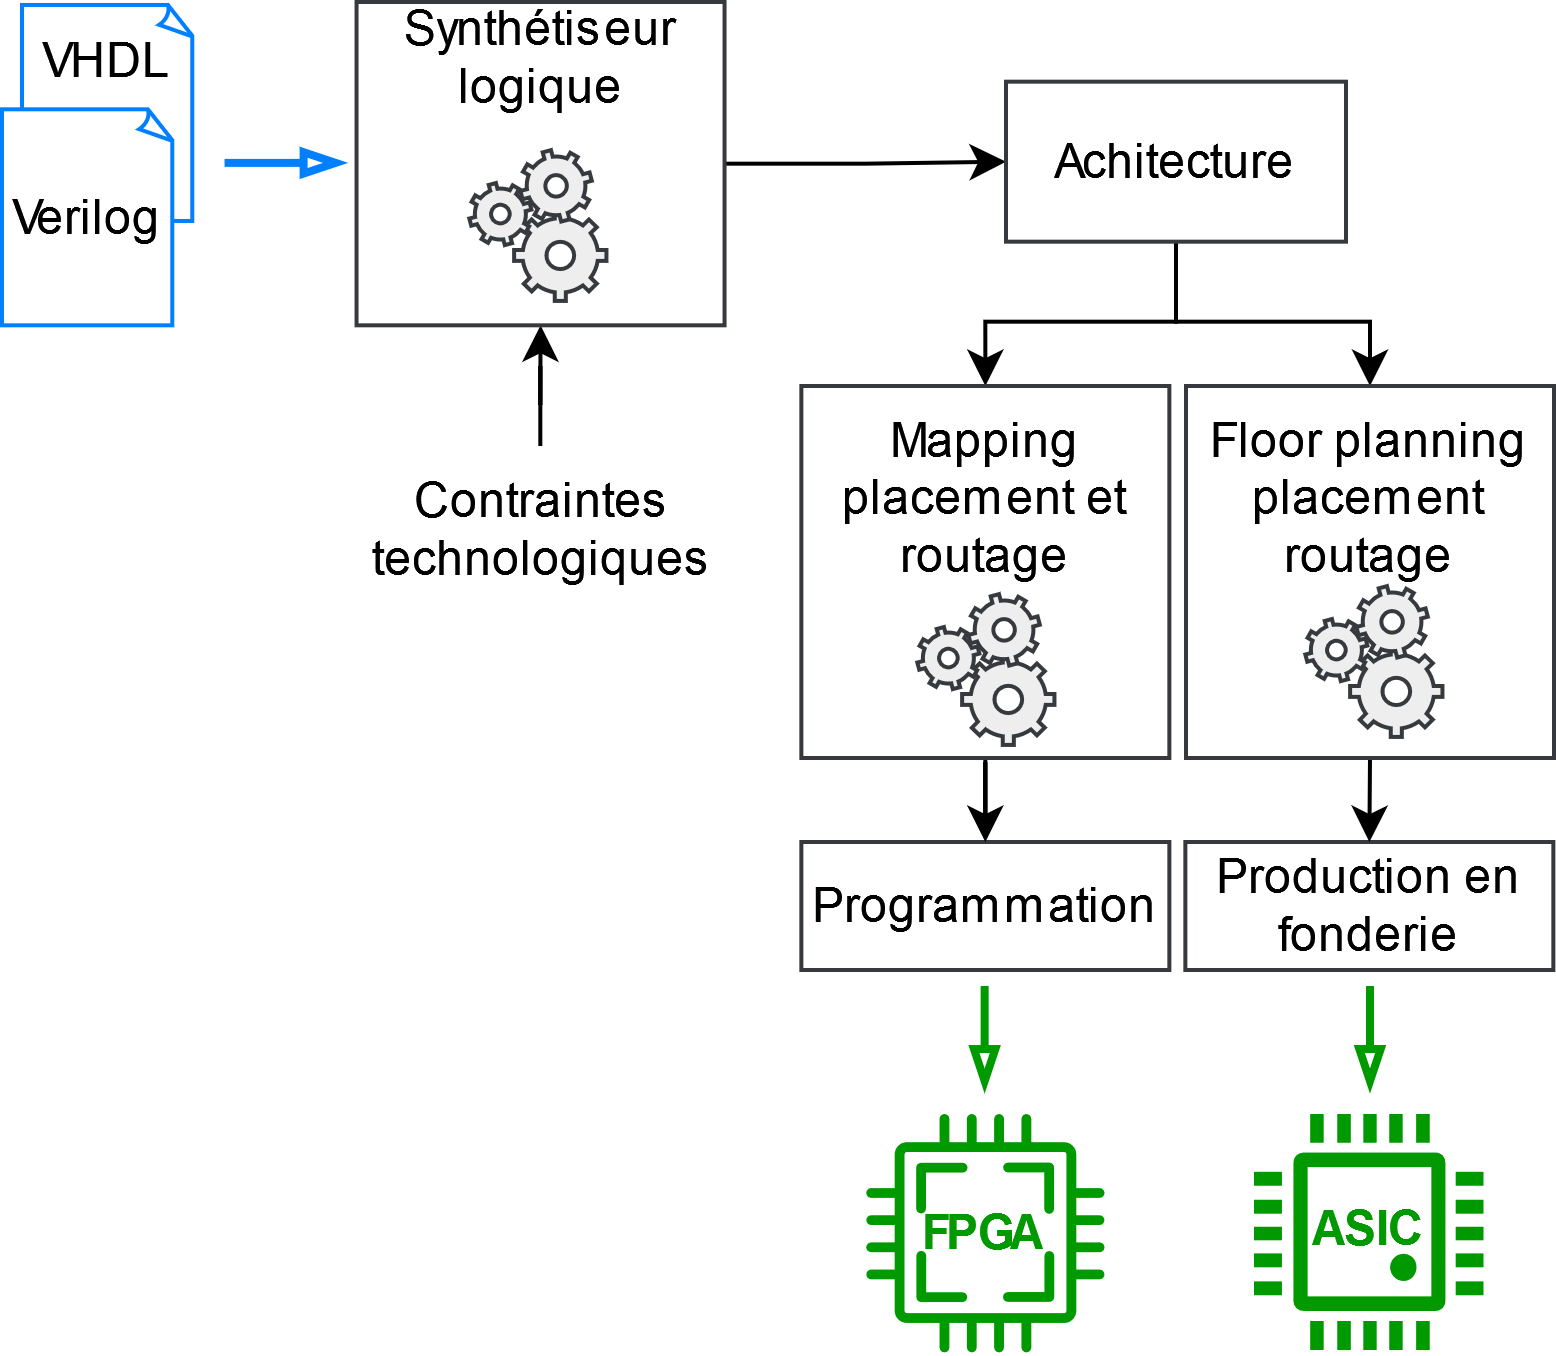
\includegraphics[scale=.13]{figs/methodo_dediee.png}
    \caption{Méthodologie de conception pour les architectures dédiées}
    \label{methodo_archi_dediees}
\end{figure}
%%%%%%%%%%%%%%%%%%%%%%%%%%%%%%%%%%%%%%%

Le manque de flexibilité et d’évolutivité des architectures dédiées sur cible ASIC a motivé les concepteurs à évaluer et adopter d’autres types de technologies tels que les circuits FPGA. À l’origine, les circuits FPGA servaient à prototyper et à valider les architectures numériques avant leur intégration dans des ASIC. Cependant, leur faculté de reconfiguration permet une évolution des systèmes dans le temps (flexibilité et évolutivité) tout en évitant les délais de production imposés par le passage en fonderie. Cette transition a été rendue possible grâce à l’augmentation de leurs capacités d’intégration qui a permis la mise au point de décodeurs CCE atteignant des débits de plusieurs Gbps \cite{PIGNOLY:MS,BOUTILLON,Wei18}.



Malgré les gains substantiels en termes de temps de mise au point et de flexibilité, la conception d’architectures dédiées sur cibles ASIC ou FPGA nécessite de longs cycles de développement. De plus, ces descriptions matérielles doivent être réécrites en fonction du débit ciblé, du format de quantification et de la taille du code (\textbf{N}). Cela implique des coûts récurrents liés aux modifications plus ou moins importantes à apporter aux architectures. Ces aspects limitent fortement l’exploration de l’espace des solutions. 


Depuis une dizaine d’années, avec les progrès réalisés par les outils de synthèse de haut-niveau (HLS), dont l’arrivée est annoncée depuis des décennies \cite{HLS1, HLS2, HLS3}, une simplification de l’exploration de l’espace des solutions et un raccourcissement des cycles de développement est possible. En effet, les outils de HLS industriels tels que Vitis HLS \cite{Vitis} ou Catapult-C \cite{catapult_c} procurent des gains majeurs en termes de productivité. Ces outils permettent, comme cela est schématisé dans la figure \ref{methodo_archi_dediees_synth_hl}, de concevoir automatiquement des architectures dédiées de niveau RTL à partir de descriptions comportementales exprimées dans des langages de haut-niveau tels que les langages C, C++ et SystemC. En plus de réduire le temps de conception d’architectures dédiées au niveau RTL, ils facilitent l’exploration de l’espace des solutions via l'utilisation d’annotations présentes dans le code comportemental et l'insertion de contraintes lors de la synthèse. 

\begin{figure}[tb]
    \centering
    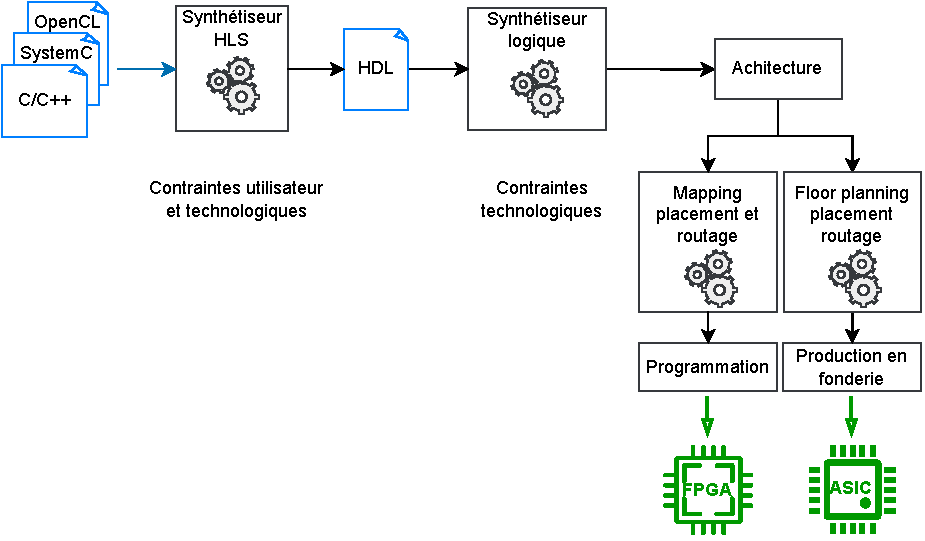
\includegraphics[scale=.9]{figs/methodo_hl.pdf}
    \caption{Méthodologie de conception intégrant la synthèse de haut niveau}
    \label{methodo_archi_dediees_synth_hl}
\end{figure}

Les différents travaux de recherche menés depuis le milieu des années 2010 ont démontré la capacité de ces méthodologies à produire des architectures de qualité comparables à celles décrites manuellement au niveau RTL. Ce résultat est dû à l'amélioration des algorithmes de synthèse intégrés à ces outils, mais également à leur capacité à être intelligemment guidés par le concepteur. Différentes études traitant de l’implantation de décodeurs CCE pour les codes LDPC \cite{HLS:LDPC1,HLS:LDPC2,HLS:LDPC3}, les codes LDPC non binaires \cite{HLS:LDPC:NB}, les turbo codes \cite{HLS:TURBO} et les codes polaires \cite{HLS:POLAR} ont mis en évidence la maturité des méthodologies basées sur les outils HLS. Toutefois, ces études ont aussi mis en lumière l’impact de la qualité des modèles comportementaux et des directives de synthèse sur les niveaux de performance atteignables : pour atteindre des niveaux de performance équivalents à celui des architectures développées au niveau RTL, il est, par exemple, nécessaire de développer des modèles comportementaux intégrant des aspects architecturaux (ex. découpage en sous-tâches) \cite{HLS:POLAR,HLS:LDPC1,HLS:LDPC2,HLS:LDPC3}. 


Ces méthodologies fondées sur les outils HLS permettent de considérablement réduire le temps de développement des décodeurs de CCE matériels. 
De plus, elles sont actuellement en phase avec l’écosystème du Cloud Computing. 
Cet écosystème est composé des servers distants, eux-mêmes constitués de plusieurs processeurs et des cartes accélératrices de type FPGA. Ainsi, l'application de méthodologies HLS dans cet écosystème permet de rapidement déployer des infrastructures de communications numériques \cite{CloudComp:1,CloudComp:2,CloudComp:3,CloudComp:4}.
Cependant, il reste difficile de produire des architectures matérielles génériques et flexibles capables, par exemple, de gérer efficacement les multiples variantes de codes LDPC présentes dans le standard 5G et/ou de supporter plusieurs familles de CCE.
%
% 
% 
% 
% 
\section{Architectures programmables}
%
% 
% 
% 
% 
Afin d’apporter des niveaux de flexibilité et d’évolutivité supérieurs et répondre aux besoins énoncés par le concept de Software Defined Radio (SDR) \cite{SDR}, au début des années 2010, de nombreuses études se sont focalisées sur le développement de chaînes de communications numériques purement logicielles. En effet, l’exécution de programmes sur des architectures programmables de type CPU ou GPU offre, d’un point de vue système, à la fois des niveaux de flexibilité et d’évolutivité élevés ainsi qu’une simplicité de mise en œuvre face à la mise au point de solutions ASIC/FPGA.



Pour déployer tout ou partie d’un système sur une architecture programmable, il est nécessaire de décrire le comportement des algorithmes à exécuter dans un langage de programmation tel que le C/C++. Ces différentes descriptions comportementales sont dans un second temps analysées, optimisées et traduites en code machine par un compilateur tel que schématisé dans la figure \ref{methodo_GPP}. Le compilateur (ex. \acrshort{gcc},Clang/LLVM), durant les phases d’optimisation et de génération du code machine, est contraint par le jeu d’instructions du processeur ciblé, mais aussi par la qualité de la description logicielle.
%%%%%%%%%%%%%%%%%%%%%%%%%%%%%%%%%%%%%%
\begin{figure}[tb]
    \centering
    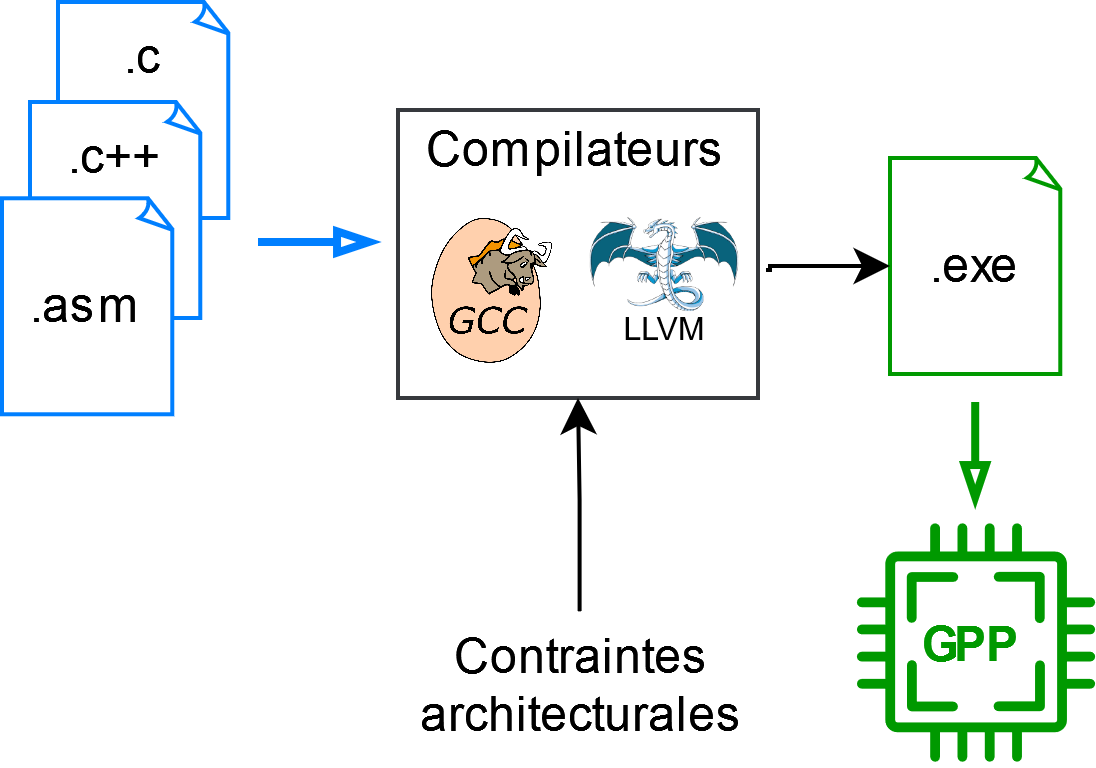
\includegraphics[scale=0.20]{figs/methodo_gpp.png}
    \caption{Flot de conception pour un processeur généraliste}
    \label{methodo_GPP}
\end{figure}
%%%%%%%%%%%%%%%%%%%%%%%%%%%%%%%%%%%%%%
Dans le but d’améliorer les performances des applicatifs, certaines parties des descriptions comportementales peuvent être décrites en assembleur afin de profiter au mieux des capacités spécifiques des processeurs (\textit{prefetch} des caches, instructions spécialisées, etc.). Même si ce travail de description et d’optimisation est un processus qui peut être long et complexe, ces durées sont incomparables avec celles nécessaires pour la conception d’architectures matérielles.
Toutefois, au début des années 2000, les puissances de calcul offertes par les architectures programmables (CPU mono-cœur et \acrshort{dsp}) étaient bien inférieures à celles nécessaires pour l’exécution temps réel des systèmes de communication. Cet état de fait restreignait l'usage des CPU à l’étude des performances des systèmes de communications numériques à l’aide de simulations de type Monte Carlo.



L’apparition d’unités de calcul vectoriel telles que les extensions MMX/SSE\footnote{Extensions multimédia du jeu d’instructions des processeurs INTEL et AMD, respectivement SIMD 64 bits et 128 bits.} dans les cœurs de processeur généraliste et dans les DSP relança l’engouement pour ce type de solution \cite{turbo:mmx,viterbi:sse,viterbi:mmx}. Cependant, ce n’est qu’avec l'arrivée des premières architectures massivement parallèles telles que l'architecture CELL \cite{CELL} produite en 2006 par Sony pour la PlayStation 3 que le concept de radio-logicielle devint envisageable  \cite{CELL:LDPC1,CELL:LDPC2,CELL:TURBO}. En effet, le processeur CELL était composé d’un cœur PowerPC traditionnel qui était couplé à 8 cœurs spécialisés. Chacun de ces cœurs possédait une unité vectorielle (Single Instruction Mulitple Data, \acrshort{simd}) capable d’exécuter 2 instructions par cycle d’horloge, chaque instruction traitant Q données (avec Q données \times  largeur des données = 128 bits).



Les premiers travaux universitaires ciblant cette architecture  \cite{CELL:LDPC1,CELL:LDPC2,CELL:TURBO} se sont focalisés sur la proposition de stratégies de parallélisation des algorithmes de décodage des CCE en phase avec les spécificités architecturales et le jeu d’instructions vectoriel à disposition. Ces études se sont concentrées sur des algorithmes de décodage CCE « naïfs » offrant un parallélisme de calcul régulier facilement accessible. Par exemple, dans le cadre du décodage des codes LDPC, l’ordonnancement par vague (flooding schedule) était préféré aux ordonnancements par couches (layered schedule) à cause de sa régularité et du fort parallélisme de calcul exposé. Couplées à l’utilisation de données flottantes, ces premières descriptions logicielles de décodeurs LDPC appliquées au standard WiMAX exploitant l’intégralité du processeur CELL permettaient d’atteindre des débits de quelques dizaines de Mbps. 



Ces travaux permirent de démontrer la viabilité du concept de Software-Defined Radio (SDR), malgré des niveaux de performances modestes en termes de débit face aux solutions ASIC/FPGA. Ils ont ensuite été étendus aux architectures multi-cœurs et many-cœurs (GPU) dont la conception et l’usage s'étaient généralisés. Les architectures de processeurs graphiques (GP-GPU) offraient de nouvelles opportunités grâce à (1) leur paradigme de programmation SIMT (Single Instruction Multiple Threads) simplifiant grandement la description des traitements à réaliser et (2) un nombre de cœurs de calcul « élémentaires » pouvant atteindre plusieurs milliers d’unités \cite{14}[13]. Ce grand nombre de cœurs de calcul associé à des fréquences de fonctionnement variant de 1 à 2 GHz semblait un choix pertinent pour l’implantation de systèmes de communications numériques, et plus particulièrement de décodeurs de CCE.



Différents langages de programmation ont été développés pour permettre de programmer ces circuits, parmi les plus connus, peuvent être cités OpenCL \cite{OpenCL} et CUDA \cite{CUDA}. Ils permettent à la fois de décrire simplement le parallélisme de calcul et d’avoir un niveau de granularité suffisant pour adapter au mieux ce parallélisme à la plateforme d’exécution. Comme cela est illustré dans la figure \ref{methodo_multimany}, le développeur doit modéliser le comportement des fonctions à accélérer à l’aide d’un langage dédié, mais il doit également écrire le code logiciel permettant au système hôte d’effectuer les transferts de données vers/depuis le GPU et d’initier les traitements.
%%%%%%%%%%%%%%%%%%%%%%%%%%%%%%%%%%%%%%
\begin{figure}[tb]
    \centering
    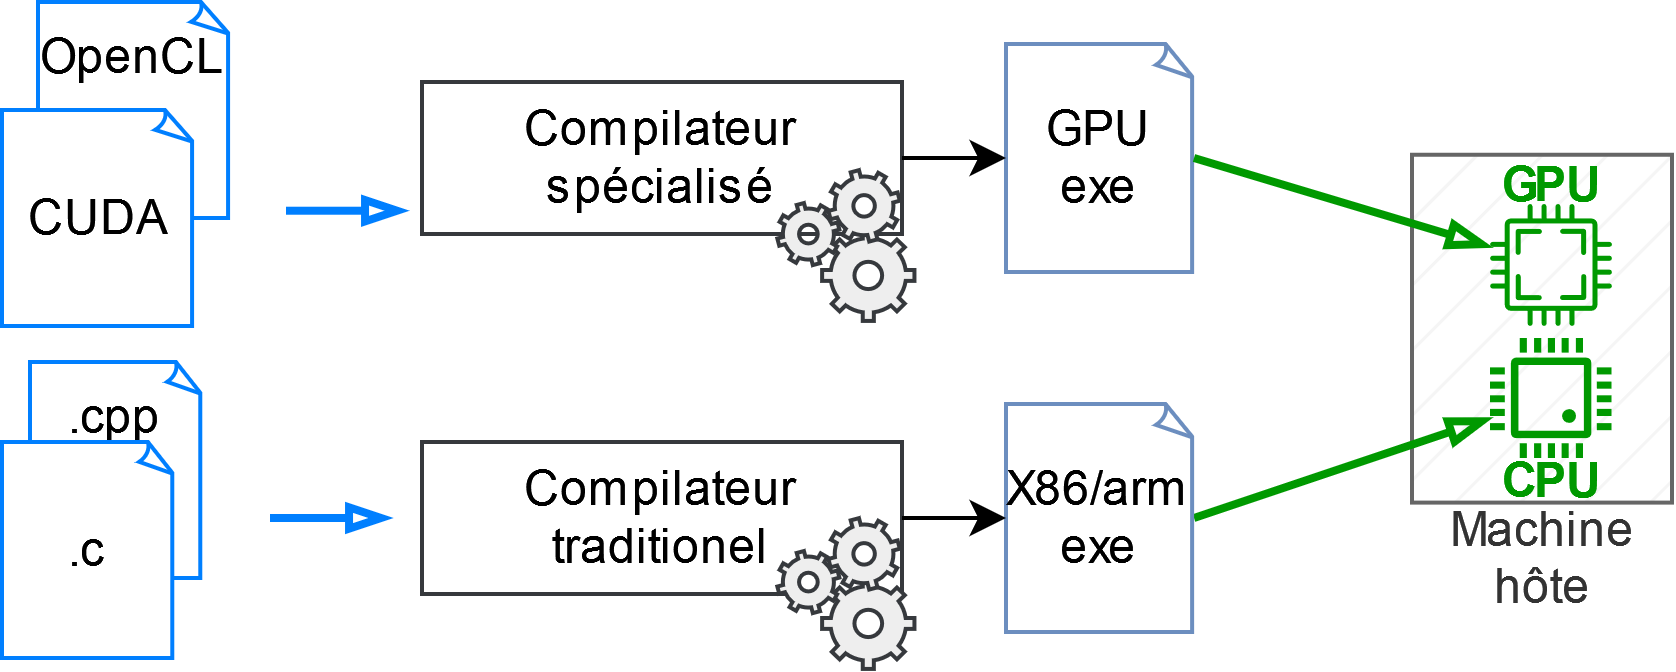
\includegraphics[scale=.17]{figs/methodo_multimany.png}
    \caption{Méthodologie de conception pour une architecture multi/many cœurs}
    \label{methodo_multimany}
\end{figure}
%%%%%%%%%%%%%%%%%%%%%%%%%%%%%%%%%%%%%%
Toutefois, même si des débits supérieurs à quelques Mbps peuvent être obtenus assez aisément \cite{Wang13,Wang11,Falcao11}, l’identification de bonnes stratégies de parallélisation associée à la conception de structures de données adaptées est nécessaire pour tirer parfaitement parti de ces architectures complexes. Cette difficulté transparaît dans de nombreux travaux menés autour du décodage des codes LDPC \cite{FALCAO:SURVEY,LDPC:SOFT4}. Les premières études ciblant des GPU \cite{Falcao11} ont mis en exergue la capacité de ces plateformes à fournir des débits de décodage supérieurs à 100 Mbps, compatibles avec les attendus de standards tels que DVB-S2 \cite{DVB:S2} et WiMAX \cite{wimax}. 
Cependant, la nature même des algorithmes de décodage de CCE possédant un parallélisme de calcul limité (LDPC, turbo codes), irrégulier (codes polaires) ou bien la nécessité de réaliser des accès non contigus à la mémoire (LDPC et turbo codes) limite l’efficacité de ce type de solution par rapport aux capacités théoriques des architectures.
Afin de saturer les centaines ou les milliers de cœurs de calcul disponibles au sein des GPU et apporter de la régularité au niveau des accès-mémoire, une solution étudiée a consisté à décoder un nombre important de trames en parallèle \cite{BLG:GPU}. Cette stratégie améliore fortement le débit, mais impacte aussi négativement la latence de traitement, rendant de facto ces solutions incompatibles avec les standards de communication mobile tels que la 4G LTE \cite{Ref_4G} et la 5G 3GPP \cite{5g}.


%%%%%%%%%%%%%%%%%%%%%%%%%%%%%%%%%%%%%%
Même si les débits sont compatibles avec les besoins applicatifs, les architectures de GPU possèdent des inconvénients rédhibitoires pour bon nombre de systèmes communicants:
\begin{enumerate}
    \item leur consommation de puissance qui dans les travaux publiés dépasse 100$\sim$200 Watts \cite{BLG:GPU},
    \item le pouvoir de correction dégradé car les décodeurs exécutent $2\times$ à $\sim$ $4\times$ moins d’itérations à iso-débit que les solutions matérielles sur circuit FPGA \cite{FALCAO:SURVEY}.
\end{enumerate}
%%%%%%%%%%%%%%%%%%%%%%%%%%%%%%%%%%%%%%
L’ensemble de ces points explique pourquoi, à l’heure actuelle, en dehors de travaux universitaires, les GPUs ne sont pas utilisés dans les solutions industrielles \cite{OpenAirInterface,INTEL:FLEXRAN} et restent cantonnés à la simulation et l’étude de systèmes \cite{NVIDIA:CNN:COM:NUM}.

En parallèle de ces travaux relatifs autour des GPU, des études sur les architectures multicœurs ont démontré que l’évolution de ces dernières (nombre de cœurs physiques, extensions des unités SIMD) permettaient l’obtention de solutions plus efficaces. Ils peuvent offrir des débits supérieurs à 1 Gbps et des latences inférieures à 100 µs avec consommations énergétiques maîtrisées. Plusieurs caractéristiques architecturales expliquent ces résultats:

\begin{itemize}
    \item Les jeux d’instruction SIMD présents dans les cœurs ARM et INTEL excellent dans l’exécution d’opérations entières (8 bits), ils peuvent traiter de 16 à 64 données en parallèle par cycles d’horloge. 
    \item Les décodeurs de CCE manipulent un nombre de données limité, ce qui leur permet d’exploiter efficacement les caches de niveau L1 et L2. Cela minimise le temps d’accès aux données durant le processus de décodage.
    \item Les processeurs multicœurs actuels ont des fréquences de fonctionnement $2\times$ à $5\times$ supérieures à celles des GPU. De plus, ce sont des cœurs superscalaires pouvant réaliser plusieurs instructions par cycle d’horloge lorsque les dépendances de données et la disponibilité des unités fonctionnelles l’autorisent.
\end{itemize}


Les premières études réalisées sur des architectures x86 fournissaient des résultats bien inférieurs à ceux obtenus sur des architectures GPU \cite{massive:gpu}. Ces résultats étaient liés à des choix algorithmiques peu pertinents et des stratégies de parallélisation peu efficaces, avec par exemple, un décodage par inondation sur des données flottantes 32 bits pour le décodage des codes LDPC \cite{Chang:ldpc}. Une seconde vague de travaux s’inspirant des algorithmes de décodage utilisés dans les architectures de décodeurs matériels a changé la donne. Par exemple, les résultats présentés dans \cite{LDPC:SOFT4} pour le décodage de codes LDPC, obtenus sur une architecture INTEL multicœurs issue d’un ordinateur portable, étaient de 3 à 100 fois supérieurs en termes de débits par rapport à l’état de l’art sur GPU.

Ces résultats ont motivé l’extension de ces études se focalisant sur les architectures multicœurs aux autres familles de CCE: les turbo codes \cite{Adrien} les codes polaires \cite{ri:LeG15a,mcgill} et les codes LDPC-NB \cite{BLG:LDPC:NB}. Pour l’ensemble de ces familles, les solutions multicœurs ont démontré des niveaux de performance en termes de débit, de latence et d’énergie plus intéressants que ceux des solutions fondées sur l’utilisation de GPU.
Afin de saturer les unités de calculs SIMD et obtenir une régularité des accès à la mémoire, ces décodeurs logiciels, contrairement aux décodeurs matériels qui se focalisent sur le parallélisme présent dans le processus de décodage d’une trame (intra-trame), utilisent le parallélisme présent lors du décodage de \textbf{Q} trames homogènes (inter-trames). Ainsi, chaque cœur décode \textbf{P} trames en parallèle avec 8 bits \times \textbf{Q} égal à la largeur de l’unité SIMD. La régularité des accès mémoire est obtenue en entrelaçant les trames en amont et en aval des états de décodage dans la figure \ref{fig:simd}.

\begin{figure}
    \centering
    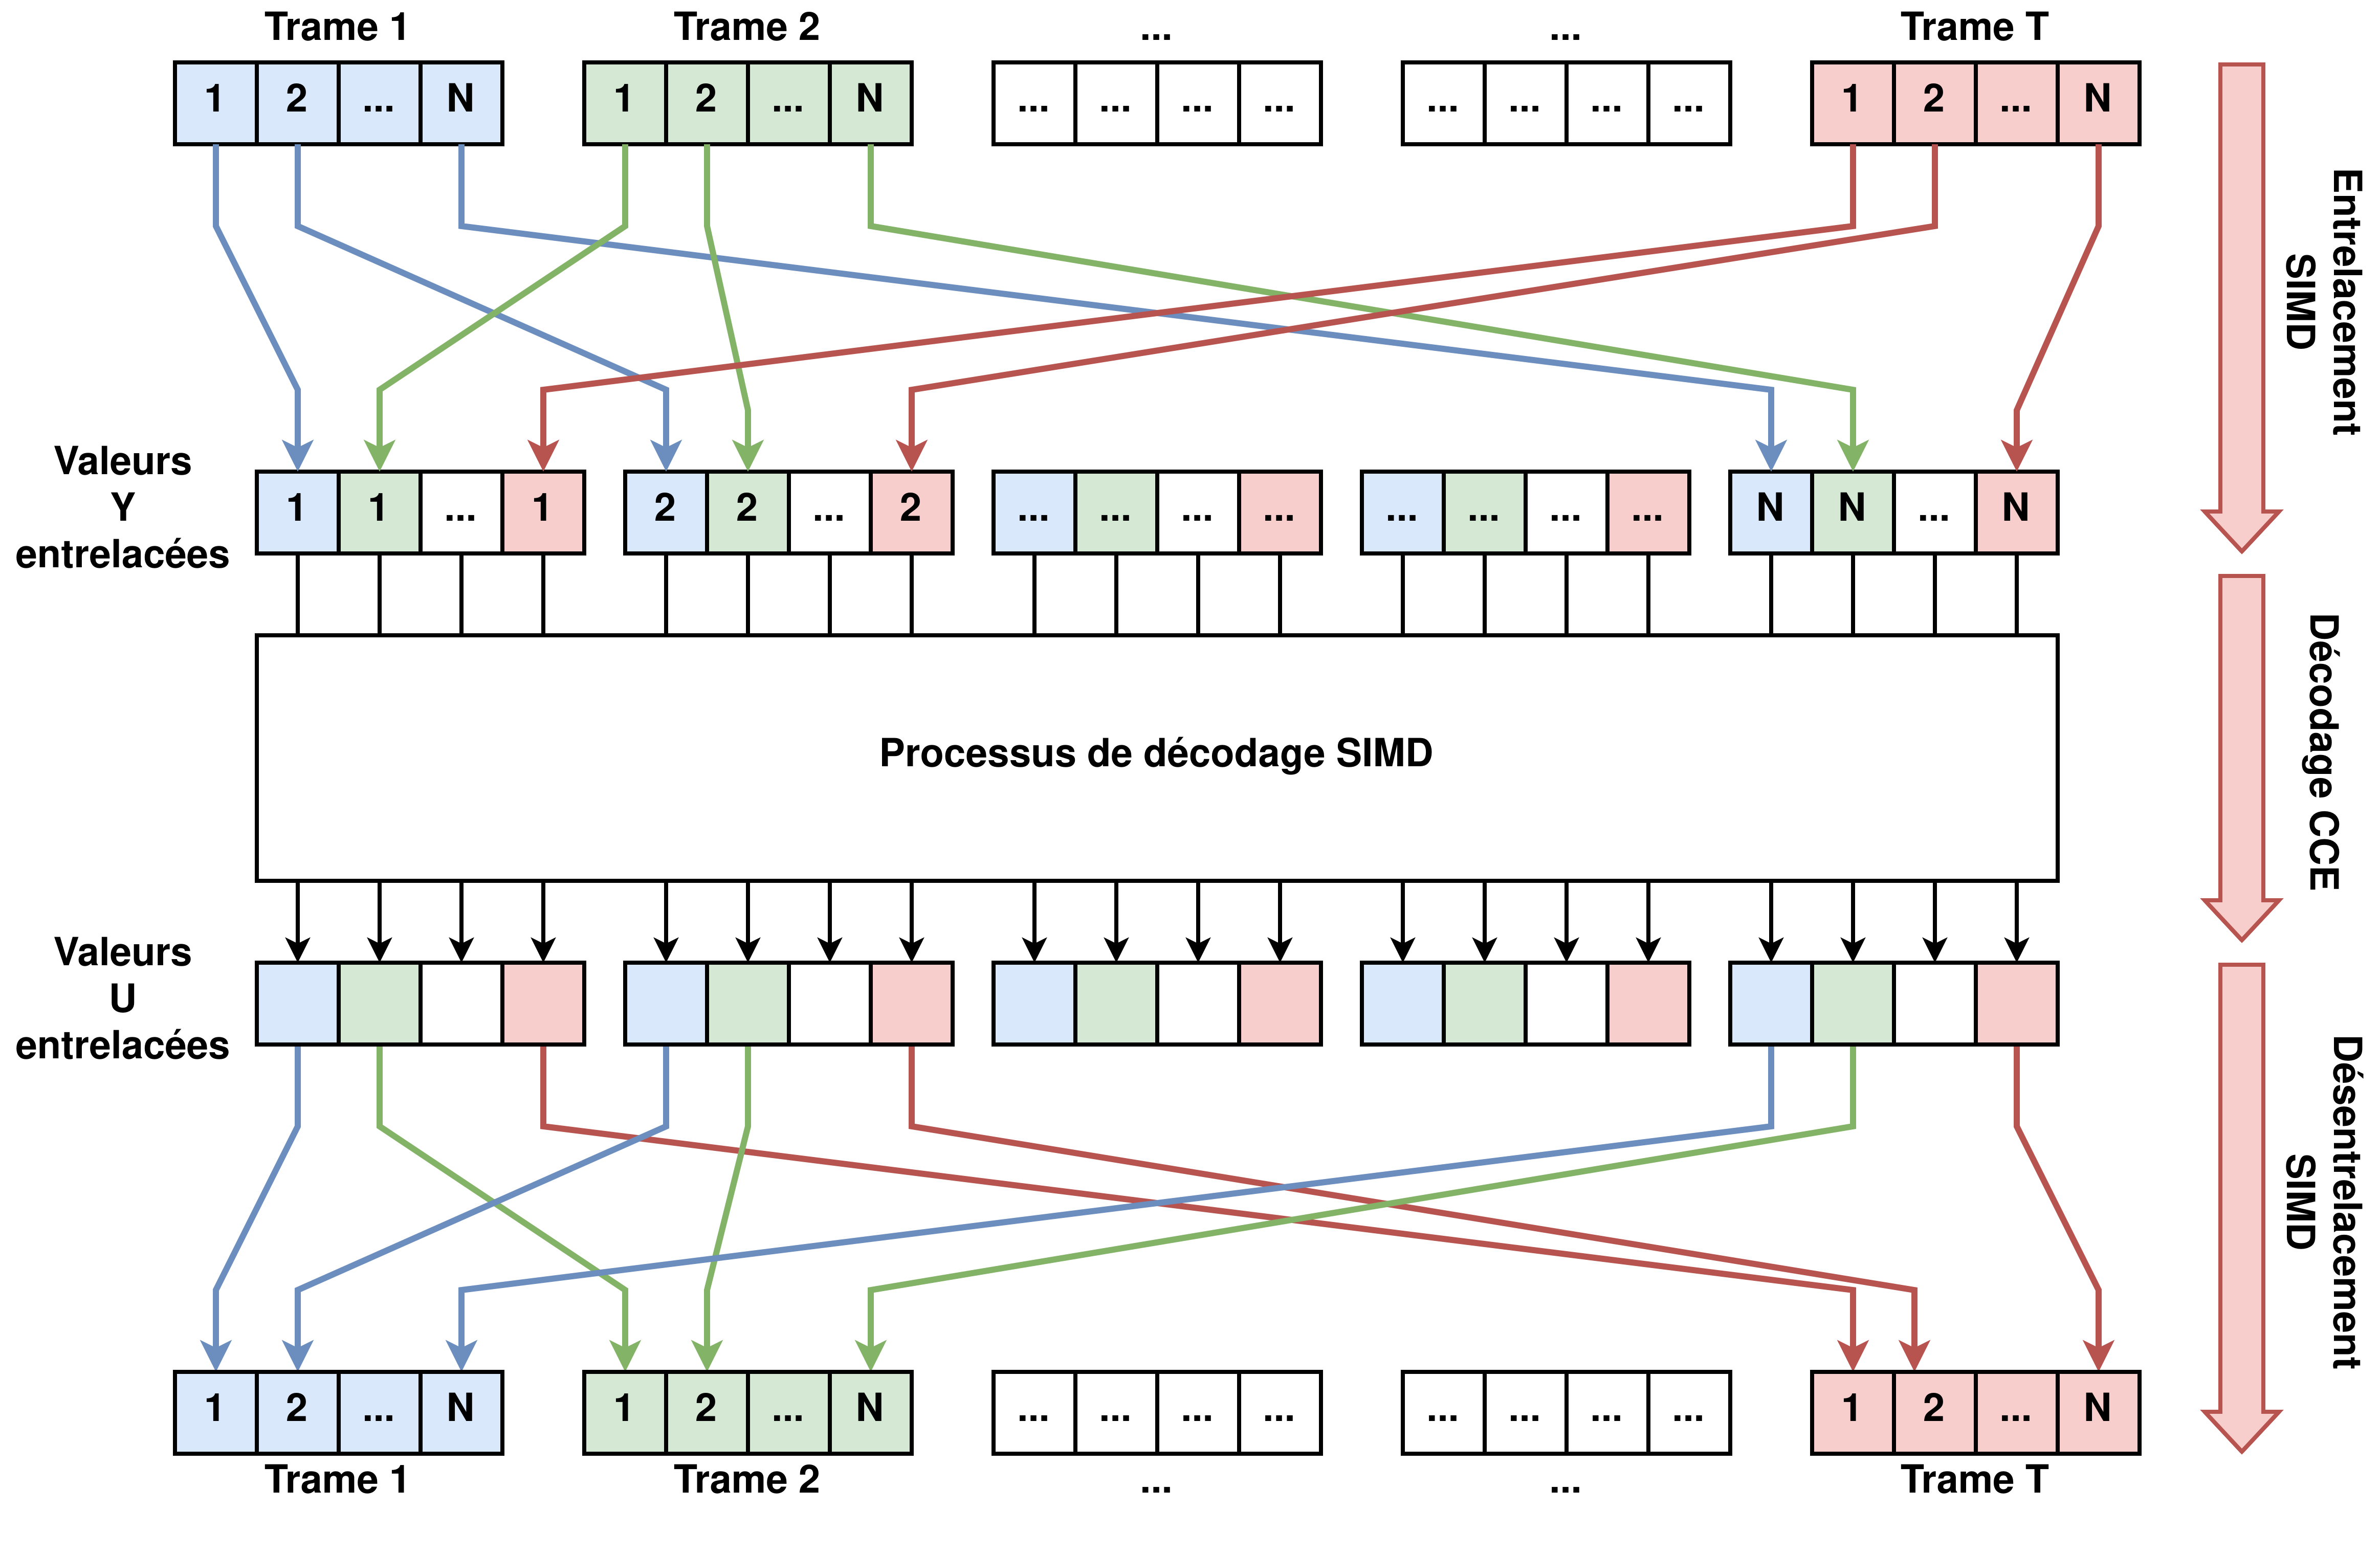
\includegraphics[scale=.08]{figs/SIMD.png}
    \caption{Procédure de décodage SIMD}
    \label{fig:simd}
\end{figure}


Ces étapes d’entrelacement, qui peuvent être accélérées grâce aux instructions SIMD des processeurs INTEL et ARM, consomment un temps d’exécution négligeable au regard du temps de décodage de CCE \cite{ri:LeG15a}. Au niveau système, chacun des \textbf{P} cœurs physiques peut décoder \textbf{Q} trames. Ces travaux de recherche ont donné naissance à la bibliothèque aff3ct \cite{aff3ct} qui a servi à concevoir, par exemple, un récepteur SDR pour le standard DVB-S2 \cite{Cass21}.


La stratégie de parallélisation inter-trames produit cependant des effets indésirables qui limitent la scalabilité de l’approche et l’intérêt réel des décodeurs :
\begin{enumerate}
    \item l’augmentation linéaire de l’empreinte mémoire avec \textbf{Q} qui provoque rapidement une saturation des caches L1/L2 lorsque $\bm{Q}$ $\in$ \{16, 32, 64\} même pour des trames de tailles modérées. À l’exécution, les performances sont limitées par la bande passante mémoire. Ainsi le facteur d’accélération plafonne et atteint une asymptote horizontale inférieure à $\bm{P} \times \bm{Q}$ lorsque l’empreinte mémoire dépasse la taille des caches L2/L3. Au niveau du système, cette utilisation de la bande passante mémoire peut aussi impacter les performances des autres traitements présents dans le récepteur.
    \item des latences de décodage (100 µs $\sim$ 10 ms) bien plus importantes que celles issues de décodeurs matériels se focalisant sur une exploitation du parallélisme intra-trame.
\end{enumerate}


L’intégration des contraintes fortes sur la latence de décodage a engendré le développement de nouveaux schémas de parallélisation \cite{BLG:SIPS:LDPC,BLG:LDPC:NB,Leonardon:2019vf,Adrien,mcgill} pour garantir le respect des valeurs attendues dans les 4G LTE \cite{Ref_4G} et 5G \cite{5g}. Ces nouvelles études ont permis de maintenir des débits de décodage élevés tout en réduisant les latences de décodage à des valeurs compatibles avec les contraintes des standards ($\leq $ 1 ms). Les implantations logicielles ont été calquées sur le comportement des architectures matérielles, tant au niveau des stratégies de parallélisation des calculs que du stockage des données. La scalabilité de l'approche est ainsi améliorée, car chaque cœur utilise son unité SIMD pour accélérer le décodage d'une seule et unique trame (parallélisation intra-trame). Cette approche diminue la pression sur les caches L2/L3 et réduit a minima d'un facteur \textbf{Q} les besoins en termes de bande passante mémoire. Comme cela est mis en évidence dans \cite{Adrien}, les débits de ces décodeurs CCE évoluent donc linéairement avec \textbf{P} et \textbf{Q}.



Malgré les progrès réalisés au niveau des architectures internes des multicœurs SIMD pour augmenter leurs performances et/ou réduire leur consommation énergétique, ces dernières restent inefficaces ($\sim 10 \times$ à $100 \times$) lorsqu’elles sont comparées à des architectures dédiées sur FPGA \cite{FAIR:LDPC}. Ce décalage est en partie lié à l’inefficacité du jeu d’instructions des processeurs multicœurs. En effet, leurs instructions sont génériques et peu adaptées aux opérations arithmétiques et logiques mises en œuvre dans les algorithmes de décodage des CCE. Ainsi, afin d’implanter les opérations élémentaires des algorithmes de décodage CCE, et ce, contrairement aux architectures dédiées où ces opérations peuvent être réalisées en un cycle d’horloge, des dizaines d’instructions peuvent être nécessaires \cite{LDPC:SOFT4}.


Afin de pallier ce facteur d’inefficacité lié à la nature intrinsèque des architectures programmables, tout en maintenant un niveau de flexibilité élevé, d’autres approches architecturales ont vu le jour. Ces dernières proposent de concevoir des cœurs de processeurs spécialisés à un domaine applicatif dans le but de rapprocher les niveaux de performance des deux mondes.
% 
% 
% 
% 
% 
\section{Architectures programmables spécifiques}
% 
% 
% 
% 
% 
L'élaboration d’architectures dédiées de décodeurs de CCE nécessite des compétences importantes dans la conception au niveau RTL et implique des cycles de développement longs. À l’opposé, l’utilisation d’architectures programmables de type processeur superscalaire ou VLIW est plus aisée et offre de la flexibilité aux concepteurs de systèmes. Cependant, leurs unités de calcul génériques ainsi que leurs jeux d’instructions limitent l’efficacité des implantations logicielles. Pour pallier cette limitation, une solution proposée au début des années 2000 \cite{XXX} et employée depuis consiste à développer des architectures de processeur spécialisées (Application Specific Instruction-set Processor – ASIP) pour un ou des domaines applicatifs. Ces cœurs de processeur, décrits à l’origine au niveau RTL, pouvaient être prototypés et déployés sur circuits FPGA ou implantés en technologie ASIC.


Les \acrshort{asip} sont donc des processeurs qui intègrent des unités de calcul dédiées à un domaine applicatif. Des instructions assembleur dédiées permettent au développeur d’exploiter ces fonctionnalités au niveau logiciel. Afin de développer ces cœurs de processeurs ASIP, différentes approches méthodologiques ont été proposées dans la littérature. La première stratégie, schématisée dans la figure \ref{fig:methodo_asip}, consiste à concevoir intégralement l’architecture pour un domaine applicatif donné \cite{ASIP:1, ASIP:2}. La paramétrisation du processeur, de ses bus de données, de ses bancs de registres et du jeu d’instructions est réalisée de manière spécifique par rapport aux besoins applicatifs. Les propriétés architecturales du processeur sont alors formalisées à l’aide d’un langage dédié (Domain Specific Language – DSL)  \cite{ASIP:DSL:1,ASIP:DSL:2,ASIP:DSL:3} ou de manière graphique \cite{ASIP:PC:SC}. Ces spécifications, une fois traitées par une suite d’outils, tels que CoWare Processor Designer \cite{Coware:1,Coware:2}, permettent la génération de:
\begin{itemize}
    \item[(a)] la description architecturale du cœur de processeur au niveau RTL;
    \item[(b)] l’environnement de développement logiciel (compilateur, debugger, etc.);
    \item[(c)] un ou des simulateurs TML/CABA couplés à des outils d’analyse.
\end{itemize}

Ce type d’approche a permis la conception de décodeurs de CCE dédiés au décodage des turbo codes \cite{Ref_FlexFEC}, des codes LDPC \cite{Ref_Flexichap} et plus récemment des codes polaires \cite{ASIP:PC:SC}. Cette garde méthodologie a permis l’obtention de niveaux de performance élevés grâce au dimensionnement au plus juste de l’architecture matérielle, cependant, elle implique des cycles de développement relativement longs.

Afin de réduire les cycles de développement et augmenter la flexibilité des architectures ASIP, une seconde approche méthodologique a émergé. Elle est basée sur la conception ou l’adaptation de cœurs de processeur existants. Cette adaptation est basée sur l'analyse logicielle des programmes à exécuter ou bien de directement depuis les fichiers binaires  \cite{PPB, PPC}. Ces approches plus génériques et fortement automatisées, comme cela est représenté dans la figure \ref{fig:methodo_asip}, tentent d’extraire des motifs d’instructions récurrents dont la factorisation sous la forme d’instructions spécialisées pourrait être bénéfique  \cite{phd_martin}. Les instructions ainsi identifiées sont ensuite ajoutées à l’architecture RTL du processeur considéré, \cite{NIOS:II}. En fonction des flots de conception, la chaîne de compilation peut être mise à jour, tout comme le code logiciel décrivant l’application. 
Ces approches permettent aux concepteurs de facilement améliorer les caractéristiques temporelles et énergétiques de leurs systèmes. Cependant, la complexité des algorithmes de détection et de sélection des motifs nécessite l’utilisation d’heuristiques pour adresser des applications réelles. Ces heuristiques associées à l’absence de connaissance a priori du domaine applicatif abouti à des niveaux de performances limités vis-à-vis d’ASIP spécifiés « manuellement ».

%%%%%%%%%%%%%%%%%%%%%%%%%%%%%
\begin{figure}[tb]
    \centering
    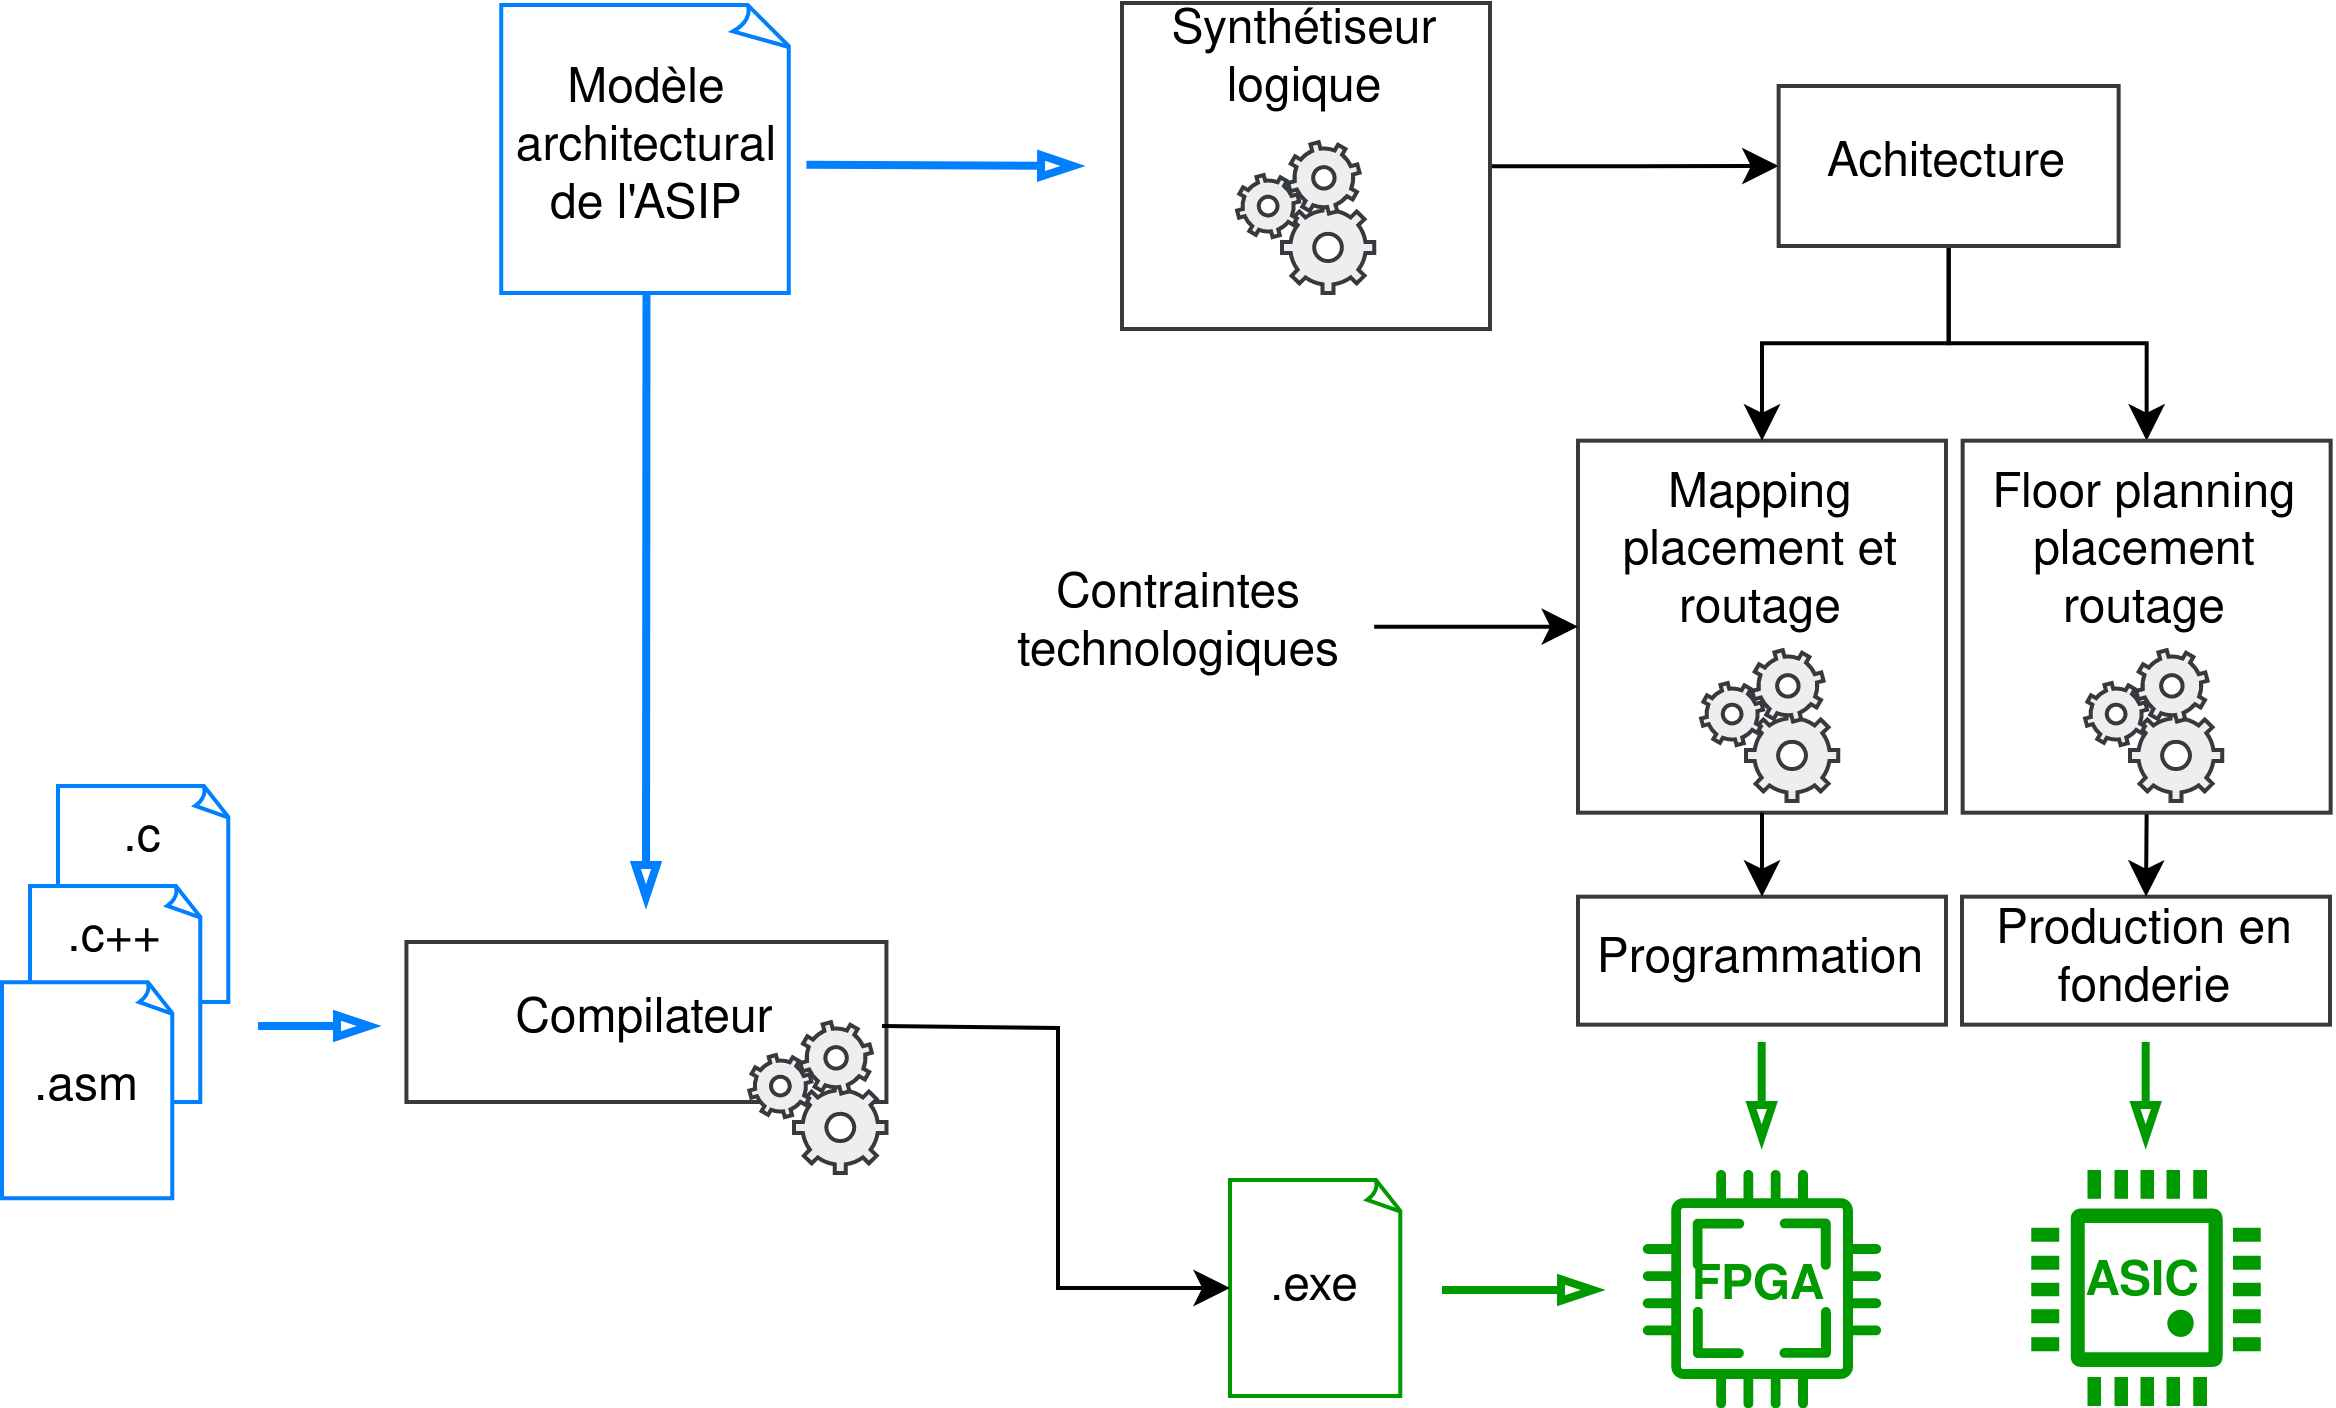
\includegraphics[scale=.15]{figs/methodo_asip.png}
    \caption{Méthodologie de conception pour ASIP}
    \label{fig:methodo_asip}
\end{figure}
%%%%%%%%%%%%%%%%%%%%%%%%%%%%%




Une troisième approche méthodologique basée à la fois sur la connaissance du domaine applicatif et sur la réutilisation de cœurs de processeur existants vise à offrir un compromis pertinent entre les performances et le temps de conception. Pour améliorer les caractéristiques des cœurs de processeurs existants, l’approche consiste à enrichir leurs jeux d’instructions à partir d’extensions liées à un ou des domaines applicatifs  \cite{INSTR:SURVEY}. Cette stratégie, basée sur les compétences du concepteur en charge de développer les extensions, a bénéficié de la démocratisation des processeurs softcore  \cite{SS1}. Ces derniers, tels que les cœurs industriels NIOS II \cite{NIOS:II} ou Xtensa  \cite{NIOS:II,XTENSA:1,XTENSA:2,XTENSA:3} permettaient aux concepteurs d’intégrer aisément leurs propres extensions.
L’avantage principal de cette approche décrite dans la figure \ref{fig:methodo_asip} réside dans le gain de temps lié à la réutilisation des architectures RTL et de leurs écosystèmes (compilateurs, debuggers, bibliothèques logicielles, etc.). Malgré la disponibilité de frameworks plus ou moins automatisés \cite{NIOS:II,XTENSA:1,phd_martin}, les capacités d’adaptation de ces approches étaient à l’origine limitées à cause de la nature propriétaire des architectures softcore et de leurs codes RTL.


L’initiative RISC-V qui vise à proposer un jeu d’instructions open-source permettant la conception de cœurs de processeurs compatibles et qui a débuté en 2010 sous l’impulsion Berkeley, a ouvert une nouvelle voie et a stimulé cet axe de recherche \cite{INSTR:SURVEY}. En effet, de nombreux cœurs de processeurs compatibles avec ISA RISC-V ont été publiés sous diverses licences open-source \cite{RISC:V:Survey,SS2}. Ainsi, ces dernières années, de nombreux travaux de recherche ont été réalisés dans le domaine afin d’identifier et de proposer des extensions au jeu d’instructions des processeurs RISC-V \cite{RISC:V:Survey} pour en améliorer l’efficience dans les domaines du traitement du signal, de la cryptographie \cite{RISC:V:AES}, de la sécurité \cite{RISC:V:FIXER} et de l’intelligence artificielle (IA) \cite{Ref_IA1}. Dans ces travaux, l’expertise des concepteurs a été mise à profit afin d’identifier les séquences d’instructions à intégrer sous la forme de nouvelles instructions. Ces études qui mesurent les avantages (accélération, consommation énergétique) et les inconvénients (coût, silicium, impact sur la fréquence) se basent sur les travaux réalisés dans le cadre de la conception d’architectures dédiées afin d’identifier les formats de données et patterns efficaces. Cependant, cette tâche n’est pas aisée, compte tenu des limitations imposées par le jeu d’instructions RISC-V. Par exemple, les instructions RV32I classiques sont contraintes à ne posséder que 2 opérandes en entrée et à produire qu’une seule donnée en sortie.

\section{Conclusions}

Dans les sous-sections précédentes, nous avons synthétisé les diverses solutions architecturales à disposition des concepteurs pour déployer tout ou partie des systèmes de communications numériques actuels. Ces solutions, en raison de leurs caractéristiques intrinsèques et des méthodologies associées, se divisent principalement en deux catégories :

\begin{itemize}
    \item[\boldsymbol{-}] \textbf{Les architectures dédiées -} elles sont conçues spécifiquement pour un applicatif ou un domaine applicatif, elles fournissent de fait des niveaux de performance élevés au détriment de la flexibilité et du temps de conception.
    \item[\boldsymbol{-}] \textbf{Les architectures programmables -} elles sont génériques et flexibles par construction. Elles permettent d’adresser rapidement une large gamme de domaines applicatifs, au détriment des performances (complexité, énergie).
\end{itemize}


Les avantages et inconvénients de ces approches, ainsi que des solutions intermédiaires, sont résumées dans \ref{tab:archis}. Cette synthèse permet de positionner ces différentes solutions accessibles aux concepteurs de systèmes de communications numériques en fonction de critères tels que la flexibilité, l'efficacité énergétique, le temps de conception, etc.

\begin{table}
    \footnotesize
    \centering
    \begin{tabular}{c|ccccccc}
        \toprule
        \multirow{2}{*}{Cible} & \multirow{2}{*}{Technologie} & \multirow{2}{*}{Performances} & \multirow{2}{*}{Latence} & Consommation & \multirow{2}{*}{flexibilité} & \multirow{2}{*}{Coût} & Effort de \\
              &             &              &         & énergétique  &             &      & mise en œuvre \\
        \bottomrule
        GPP                     & ASIC  & $+$  & $+$  & $++$ & $++$ & $-$  & $-$ \\
        SoftCore                & FPGA  & $+$  & $+$  & $++$ & $++$ & $-$  & $-$ \\
        GPU                     & ASIC  & $++$  & $++$ & $+$  & $++$ & $+$  & $+$ \\
        \bottomrule
        \multirow{2}{*}{ASIP}   & FPGA & $++$   & $+$  & $+$  & $+$  & $+$  & $+$ \\
                                & ASIC & $++$   & $+$  & $+$  & $+$  & $+$  & $+$ \\
        \bottomrule
        \multirow{2}{*}{Dédiée} & ASIC & $++++$ & $--$ & $-$  &      & $++$ & $+++$ \\
                                & FPGA & $++++$ & $--$ & $-$  &      & $++$ & $+++$ \\
        
        \bottomrule
    \end{tabular}
    \caption{Caractérisation des différentes méthodologies de conception de systèmes embarqués}
    \label{tab:archis}
\end{table}

L’ensemble des approches présentées dans le tableau \ref{tab:archis} permet actuellement de concevoir des systèmes embarqués communicants adaptés aux besoins des applications de type Software-defined radio (SDR). Toutefois, en fonction de leurs caractéristiques intrinsèques, elles ne sont pas toutes interchangeables en fonction des domaines applicatifs (IoT, Cloud-RAN, etc).

Cependant, depuis plusieurs années, on observe une augmentation forte de l'utilisation de solutions purement logicielles dans la conception d'infrastructures de systèmes de communication. Cela s'explique comme cela a été évoqué par la flexibilité et l'évolutivité de ces solutions ainsi que leur passage à l'échelle (scalabilité). Néanmoins, malgré ces avantages, ces solutions basées sur l'utilisation de multicœurs SIMD ou de GPU restent en retrait lorsque les systèmes sont contraints énergétiquement. Cette sous-optimalité est principalement liée à l'inadéquation du jeu d'instructions de ces architectures programmables vis-à-vis des besoins applicatifs. Des opérations simples à réaliser matériellement peuvent ainsi nécessiter de longues séquences d'instructions élémentaires, annulant de facto le gain apporté par leurs fréquences de fonctionnement élevées.  

Afin de modifier cet état de fait, nous avons décidé dans le cadre de cette thèse de nous intéresser à la proposition d'instructions adaptées au décodage des CCE usuels. Ces instructions, pouvant être intégrées dans les ISA usuelles, visent à améliorer le support des algorithmes de décodage des CCE sur les architectures programmables. Les chapitres suivants présentent diverses extensions qui permettront d'améliorer le support des CCE usuels, mais aussi de supporter différents schémas de parallélisation dédiés à l'augmentation du débit de communication (inter-trames) et/ou à la réduction de la latence (intra-trames).

\end{document}